%%%%%%%%%%%%%%%%%%%%%%%%%%%%%%%%%%%%%%%%%%%%%%%%%%%%%%%%%%%%%%%%%%%%%
%% This is a (brief) model paper using the achemso class
%% The document class accepts keyval options, which should include
%% the target journal and optionally the manuscript type. 
%%%%%%%%%%%%%%%%%%%%%%%%%%%%%%%%%%%%%%%%%%%%%%%%%%%%%%%%%%%%%%%%%%%%%
\documentclass[journal=jcisd8,manuscript=article]{achemso}

%%%%%%%%%%%%%%%%%%%%%%%%%%%%%%%%%%%%%%%%%%%%%%%%%%%%%%%%%%%%%%%%%%%%%
%% Place any additional packages needed here.  Only include packages
%% which are essential, to avoid problems later. Do NOT use any
%% packages which require e-TeX (for example etoolbox): the e-TeX
%% extensions are not currently available on the ACS conversion
%% servers.
%%%%%%%%%%%%%%%%%%%%%%%%%%%%%%%%%%%%%%%%%%%%%%%%%%%%%%%%%%%%%%%%%%%%%
\usepackage{amsmath}
\usepackage{graphicx}
\usepackage{siunitx}
\usepackage{chemfig}
\usepackage[version=4]{mhchem}
\usepackage{booktabs}
\usepackage{subcaption}

%%%%%%%%%%%%%%%%%%%%%%%%%%%%%%%%%%%%%%%%%%%%%%%%%%%%%%%%%%%%%%%%%%%%%
%% If issues arise when submitting your manuscript, you may want to
%% un-comment the next line.  This provides information on the
%% version of every file you have used.
%%%%%%%%%%%%%%%%%%%%%%%%%%%%%%%%%%%%%%%%%%%%%%%%%%%%%%%%%%%%%%%%%%%%%
%%\listfiles

%%%%%%%%%%%%%%%%%%%%%%%%%%%%%%%%%%%%%%%%%%%%%%%%%%%%%%%%%%%%%%%%%%%%%
%% Place any additional macros here.  Please use \newcommand* where
%% possible, and avoid layout-changing macros (which are not used
%% when typesetting).
%%%%%%%%%%%%%%%%%%%%%%%%%%%%%%%%%%%%%%%%%%%%%%%%%%%%%%%%%%%%%%%%%%%%%
\setchemfig{angle increment=30,atom sep=2em}

%%%%%%%%%%%%%%%%%%%%%%%%%%%%%%%%%%%%%%%%%%%%%%%%%%%%%%%%%%%%%%%%%%%%%
%% Meta-data block
%% ---------------
%% Each author should be given as a separate \author command.
%%
%% Corresponding authors should have an e-mail given after the author
%% name as an \email command. Phone and fax numbers can be given
%% using \phone and \fax, respectively; this information is optional.
%%
%% The affiliation of authors is given after the authors; each
%% \affiliation command applies to all preceding authors not already
%% assigned an affiliation.
%%
%% The affiliation takes an option argument for the short name.  This
%% will typically be something like "University of Somewhere".
%%
%% The \altaffiliation macro should be used for new address, etc.
%% On the other hand, \alsoaffiliation is used on a per author basis
%% when authors are associated with multiple institutions.
%%%%%%%%%%%%%%%%%%%%%%%%%%%%%%%%%%%%%%%%%%%%%%%%%%%%%%%%%%%%%%%%%%%%%
\author{Alexander Moriarty}
\email{alexander.moriarty.21@ucl.ac.uk}
\author{Takeshi Kobayashi}
\author{Matteo Salvalaglio}
\author{Panagiota Angeli}
\author{Alberto Striolo}
\affiliation[UCL]{Department of Chemical Engineering, University College London, UK}
\alsoaffiliation[UO]{School of Chemical, Biological and Materials Engineering, University of Oklahoma, USA}
\author{Ian McRobbie}
\affiliation[Innospec]{Innospec Ltd., Ellesmere Port, UK}

%%%%%%%%%%%%%%%%%%%%%%%%%%%%%%%%%%%%%%%%%%%%%%%%%%%%%%%%%%%%%%%%%%%%%
%% The document title should be given as usual. Some journals require
%% a running title from the author: this should be supplied as an
%% optional argument to \title.
%%%%%%%%%%%%%%%%%%%%%%%%%%%%%%%%%%%%%%%%%%%%%%%%%%%%%%%%%%%%%%%%%%%%%
\title{Analyzing the Accuracy of CMC Predictions using Deep Learning}

%%%%%%%%%%%%%%%%%%%%%%%%%%%%%%%%%%%%%%%%%%%%%%%%%%%%%%%%%%%%%%%%%%%%%
%% Some journals require a list of abbreviations or keywords to be
%% supplied. These should be set up here, and will be printed after
%% the title and author information, if needed.
%%%%%%%%%%%%%%%%%%%%%%%%%%%%%%%%%%%%%%%%%%%%%%%%%%%%%%%%%%%%%%%%%%%%%
\abbreviations{CMC,ML,GNN,GP,ECFP}
\keywords{Critical micelle concentration, machine learning, molecular modeling, molecules, neural networks, uncertainty quantification, molecular cartography}

%%%%%%%%%%%%%%%%%%%%%%%%%%%%%%%%%%%%%%%%%%%%%%%%%%%%%%%%%%%%%%%%%%%%%
%% The manuscript does not need to include \maketitle, which is
%% executed automatically.
%%%%%%%%%%%%%%%%%%%%%%%%%%%%%%%%%%%%%%%%%%%%%%%%%%%%%%%%%%%%%%%%%%%%%
\begin{document}

%%%%%%%%%%%%%%%%%%%%%%%%%%%%%%%%%%%%%%%%%%%%%%%%%%%%%%%%%%%%%%%%%%%%%
%% The "tocentry" environment can be used to create an entry for the
%% graphical table of contents. It is given here as some journals
%% require that it is printed as part of the abstract page. It will
%% be automatically moved as appropriate.
%%%%%%%%%%%%%%%%%%%%%%%%%%%%%%%%%%%%%%%%%%%%%%%%%%%%%%%%%%%%%%%%%%%%%
\begin{tocentry}
    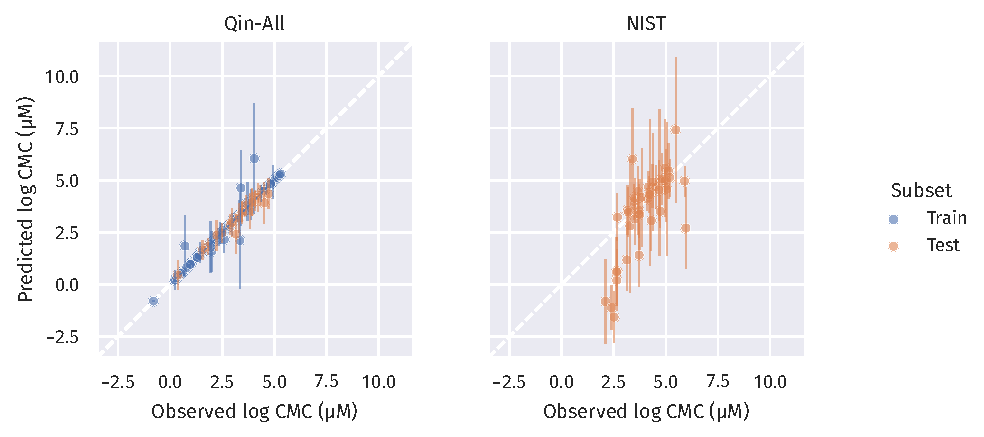
\includegraphics[width=\textwidth]{images/uq-parity.pdf}
\end{tocentry}

%%%%%%%%%%%%%%%%%%%%%%%%%%%%%%%%%%%%%%%%%%%%%%%%%%%%%%%%%%%%%%%%%%%%%
%% The abstract environment will automatically gobble the contents
%% if an abstract is not used by the target journal.
%%%%%%%%%%%%%%%%%%%%%%%%%%%%%%%%%%%%%%%%%%%%%%%%%%%%%%%%%%%%%%%%%%%%%
\begin{abstract}
    This paper presents a novel approach to predicting critical micelle
    concentrations (CMCs) using graph neural networks (GNNs) augmented with
    Gaussian processes (GPs). The proposed model uses learned latent space
    representations of molecules to predict CMCs and estimate uncertainties. The
    performance of the model on a dataset containing nonionic, cationic, anionic
    and zwitterionic molecules is compared against a linear model that works
    with extended-connectivity fingerprints (ECFPs). The GNN-based model
    performs slightly better than the linear ECFP model, when there is enough
    well-balanced training data, and achieves predictive accuracy that is
    comparable to published models that were evaluated on a smaller range of
    surfactant chemistries. We illustrate the applicability domain of our model
    using a molecular cartogram to visualize the latent space, which helps
    identify molecules for which predictions are likely to be erroneous. The
    proposed approach can provide valuable insights into the molecular
    properties that influence CMCs.
\end{abstract}

%%%%%%%%%%%%%%%%%%%%%%%%%%%%%%%%%%%%%%%%%%%%%%%%%%%%%%%%%%%%%%%%%%%%%
%% Start the main part of the manuscript here.
%%%%%%%%%%%%%%%%%%%%%%%%%%%%%%%%%%%%%%%%%%%%%%%%%%%%%%%%%%%%%%%%%%%%%
\section{Introduction}

The critical micelle concentration (CMC) of a surfactant defines the
concentration above which the surfactant monomers self-assemble in solution to
form micelles. It is an important property because the formation of micelles
affects many interfacial phenomena
\cite{rosenSurfactantsInterfacialPhenomena2012} and because micelles can
encapsulate hydrophobic molecules to form useful complexes. However, predicting
the CMC for an arbitrary chemical structure remains challenging.

Perhaps the most well-established predictor for CMC, $X_{cmc}$, is the Stauff-Klevens relationship, first published in \citeyear{klevensStructureAggregationDilate1953} \cite{klevensStructureAggregationDilate1953}. It formalised the observation that CMC decreases exponentially with an increase in the number of carbons in the hydrocarbon tail, $n_c$:

\begin{equation}
    \label{eq:klevens}
    \log X_{cmc} = A - Bn_c, \quad B > 0
\end{equation}

where $A$ and $B$ are empirical constants that depend on the temperature and the homologous series, i.e. the headgroup. The model is simple yet accurate, and it is easily interpretable: to reduce CMC, it is sufficient to extend the surfactant's hydrocarbon tail thus defining an easy-to-apply qualitative heuristic. Its drawback as a predictive model is its very limited applicability domain; each set of parameters is only applicable to surfactants with a specific headgroup and a linear carbon tail.

There have been a wealth of investigations into making more general models for
CMC prediction; here, a brief review of some diverse and promising approaches
for predicting CMCs of aqueous, single-surfactant systems will be given.

Broadly, CMC predictive models take four forms: empirical, semi-empirical,
theoretical and simulated, or some combination of these. Here we will focus on
predictive models for aqueous solutions containing a single surfactant and
discuss some of the trade-offs between the different approaches with regards to
speed, universality and interpretability.

Theoretical approaches have the potential to be the most useful type of
predictive model, if they are accurate and applicable to the desired system, as
they are directly related to scientific knowledge and their results can be
understood in terms of well studied principles.
\citet{puvvadaMolecularThermodynamicApproach1990} derived a phenomenological
model for studying aqueous nonionic surfactant systems that enabled CMC
prediction, as well as modelling of other properties across a range of
temperatures. The model they developed was the product of decomposing the
process of micellisation into discrete steps that they could describe
thermodynamically so as to yield an description of the free energy of
micellisation in terms of a set of molecular parameters:

\begin{itemize}
    \item The tail length, described as the number of carbon atoms.
    \item The average cross-sectional area of the headgroup, which controls the
          steric contribution to the free energy. This must be estimated.
    \item The Tolman length of the tail, which effectively describes the
          thickness of an `interaction region' around the tail
          \cite{demiguelGibbsThermodynamicsSurface2021}. This must also be estimated.
\end{itemize}

A functional form to estimate the parameters was described for linear, nonionic,
polyoxyethylene alcohol surfactants. The model attained impressive accuracy for
some predictions: a root-mean-squared error (RMSE) of approximately
\SI{0.14}{\log \micro M} for the group \ce{C10E_i}, where $i \in [3, 6]$, and
\SI{0.21}{\log \micro M} for the group \ce{C12E_j}, where $j \in [3, 8]$.
However, for other systems, like \ce{C8E6}, the error is much larger. The
authors expect that this inaccuracy is because the model overestimates the CMC
values for systems in which the micelles do not grow.

The connection that this model established between a small set of physically
meaningful properties that can be estimated and emergent properties of
surfactants is extremely useful, especially because it does not explicitly
require fitting to any experimental data. However, the procedures described for
estimating the Tolman length are only applicable for linear hydrocarbon chains;
not the branched case, or for heterogeneous tail groups. Estimating the average
cross-sectional area of the head group may also not be trivial.

Semi-empirical approaches are grounded in theory, but have parameters that are
optimised based on experimental data. Many semi-empirical approaches to CMC
prediction can be described as \emph{segment-based} methods, whereby the
surfactant is decomposed into discrete segments which correspond to groups of
atoms and bonds.

\citet{liStudiesUNIQUACSAFT1998} applied a segment-based UNIQUAC model
(s-UNIQUAC) and a SAFT equation of state to predict CMCs of linear
polyoxyethylene alcohols, by first deriving expressions for the activity
coefficient of a surfactant in water. In the s-UNIQUAC model, a segment-based
local-composition model was used and the fugacity could then be approximated
using the fitted interaction energies between the segments and water. In this
case, the segments used were \ce{C2H4} and \ce{C2H4O}. In the SAFT approach, the
surfactant was treated as a chain of soft-sphere segments in order to first
derive the Helmholtz energy of the solution and from that to derive the
fugacity. In this case, the segments used were \ce{CH2}/\ce{CH3} (these were
treated as the same segment) and \ce{C2H4O}. The interaction energies of the
segments were fitted, as well as parameters of a function describing the soft
sphere diameter of a segment in a chain in terms of the chain length.

\citet{chengCorrelationCriticalMicelle2005} compared the performance of these
models on a larger dataset, alongside three other models. Two of these were
segment-based models: the polymer-NRTL model \cite{liStudiesUNIQUACSAFT1998} and
a UNIFAC model \cite{voutsasPredictionCriticalMicelle2001}, both of which were
cited as inspirations for the s-UNIQUAC model. The authors also employed their
own modified Aranovich and Donohue (m-AD) model. The m-AD model calculates the
CMC as a mole fraction, $x_S^L$, approximating it as the reciprocal of the
limiting value of the surfactant's activity coefficient in aqueous solution,
$\gamma_S^{L,\infty}$:

\begin{equation}
    \label{eq:m-AD}
    x_S^L = \frac{1}{\gamma_S^{L,\infty}}
\end{equation}

The m-AD model considers the exchange equilibrium on a three-dimensional lattice
of infinitely separated solvent and solute molecules in order to determine
$\gamma_S^{L,\infty}$. Notably, the m-AD model is not a segment-based model.
Instead, the authors fitted an interchange energy, $\Delta$, separately for each
molecule. Of course, if a new parameter must be fitted for every molecule, a
model has no predictive ability. Therefore, correlations were examined between
$\Delta$ and other, readily calculated surfactant properties, which will be
discussed later.

Where data from literature was available, the predictive performance of the
models on the molecular series \ce{C_nE6}, \ce{C_nE8}, \ce{C_nE9}, \ce{C10E_n}
and \ce{C12E_n} were compared, and the resulting RMSEs are summarised in Table
\ref{tab:segment-methods}.

\begin{table}
    \caption{Comparison of the RMSEs of selected models on polyoxyethylene
        alcohols. Data from \citet{chengCorrelationCriticalMicelle2005}.}
    \label{tab:segment-methods}
    \begin{tabular}{lr}
        \toprule
        \multicolumn{1}{c}{Model} & \multicolumn{1}{c}{RMSE (\si{\log \micro M})} \\\midrule
        p-NRTL                    & 0.18                                          \\
        s-UNIQUAC                 & 0.14                                          \\
        SAFT                      & \textbf{0.06}                                 \\
        UNIFAC                    & 0.14                                          \\
        m-AD                      & 0.11                                          \\\bottomrule
    \end{tabular}
\end{table}

TODO: Talk about geometric, topological and electronic descriptors, as well as
simulation approaches.

Here, we build upon this previously published GNN model in two ways: we apply a
hyperparameter search algorithm to further optimise the model's architecture and
improve its accuracy, and we implement an \emph{uncertainty quantification}
technique that yields confidence intervals alongside CMC predictions. This
improved model is compared against an adaptation of the group contribution
approach that determines the entire set of groups to consider using a feature
selection routine. In addition, a separate dataset is introduced so as to
perform external validation and to probe the limits of the models' applicability
domain, as well as to analyse the uncertainty quantification. Finally, we
discuss methods to interpret both models, and demonstrate a technique that
allows one to visualise chemical space through the `eyes' of the trained GNN. We
show that this technique facilitates a better understanding of the applicability
domain.

\section{Method}

\newcommand{\lrv}{\vec{v}^{\,(p)}}

Two datasets were used for training and testing:

\begin{description}
    \item[The Qin dataset] is a dataset of 202 surfactants curated by
          \citet{qinPredictingCriticalMicelle2021}. To the authors' knowledge,
          it is currently the largest public dataset of CMCs for several classes
          of surfactant collected at standard conditions in an aqueous
          environment between \SIrange{20}{25}{\celsius}. In this work, the data
          was further subdivided into two tasks: Qin-All, the entirety of the
          dataset, and Qin-Nonionics, which contains only the nonionic
          surfactants.

          The Qin data were split into training and test subsets; the training
          data were used to fit the models, whilst test data were `locked away'.
          The performance metrics on the test data were used for evaluation of
          the models derived here. For some models, the training data were
          further split into optimisation and validation subsets; the
          optimisation data were used when calculating the loss function during
          model fitting. The validation data were used for on-the-fly evaluation
          of model performance during training, to determine how many iterations
          of the optimisation routine to use.

          To provide a consistent benchmark of model performance with
          the previous work \cite{qinPredictingCriticalMicelle2021}, the same
          train/test data splits were used as
          \citet{qinPredictingCriticalMicelle2021}. This will be referred to as
          the benchmarking test.

          After training these models, a sensitivity analysis was carried out.
          The data for each task were split using a repeated, stratified
          $k$-fold cross-validation. Each molecule was assigned a class based
          upon its molecular fingerprint, which will be described below, in the
          section on Extended connectivity fingerprints. The data were then
          split into $k$ folds of roughly equal size, and containing
          approximately the same percentage of molecules of each class, for $k
          \in (2, 5)$. For each fold, a model was trained using $k-1$ folds and
          evaluated on the remaining fold. This was repeated thrice for $k = 2$
          and twice for $k = 3$, each time with different randomisation, and
          there were no repetitions for $k = 4$ and $k = 5$, so that there were
          a similar number of models trained for each value of $k$.

    \item[The National Institute of Science and Technology (NIST) dataset]
          contains 43 unique surfactant systems and their aqueous CMCs,
          extracted from the work of
          \citet{mukerjeeCriticalMicelleConcentrations1971}. The original
          document compiles CMC measurements for each system across several
          temperatures and with various additives. Each measurement was given a
          quality rating depending on the authors' assessment of the
          experimental method; measurements with a sufficiently good rating were
          categorised as `suggested' measurements. The dataset used for this
          work was developed by taking the mean of the suggested CMC
          measurements between \SIrange{20}{25}{\degreeCelsius}, with no
          additives. The surfactant systems that contained elements that were
          not present in the dataset (\ce{Mn}, \ce{Cs} and \ce{Mg}) were then
          pruned. The dataset is provided in the Supplementary Information.

          The NIST data were used exclusively for external validation. Several
          of the surfactant systems in the dataset are not expected to be within
          the applicability domain of the models derived here. This includes
          surfactants with counterions and combinations of functional groups
          that are not present in the training data. These data are included to
          test the robustness of the uncertainty quantification approach.
\end{description}

The number of each type of surfactant in the train and test subsets of the data are shown in Table~\ref{tab:data-split}. Only the models trained on the Qin-All dataset were evaluated on the NIST dataset, as it contained ionic compounds.

\begin{table}
    \centering
    \caption{The number of each type of surfactant contained in the train/test subsets of the CMC datasets. Missing entries mean no samples of that class.}
    \label{tab:data-split}
    \begin{tabular}{@{}llrrrr@{}} \toprule \multicolumn{2}{c}{Data subset} & \multicolumn{4}{c}{Number of}                                                    \\\cmidrule(r){1-2}\cmidrule(l){3-6}
               Task                                                    & Train/test                    & Nonionics & Anionics & Cationics & Zwitterionics \\\midrule
               Qin-All                                                 & Train                         & 110       & 30       & 31        & 9             \\
                                                                       & Test                          & 12        & 4        & 4         & 2             \\
               Qin-Nonionics                                           & Train                         & 110       &          &           &               \\
                                                                       & Test                          & 12        &          &           &               \\
               NIST                                                    & Train                         &           &          &           &               \\
                                                                       & Test                          & 12        & 23       & 6         & 2             \\\bottomrule
    \end{tabular}
\end{table}

The QSPR pipeline needs molecular descriptors and a functional form. The design
processes for these are called \emph{feature engineering} and \emph{model
selection}, respectively.

\subsection{Feature engineering}

In this work, two types of molecular descriptors are employed: extended
connectivity fingerprints (ECFPs)
\cite{rogersExtendedConnectivityFingerprints2010} and molecular graphs.

\subsubsection{Extended connectivity fingerprints (ECFPs)}

In the ECFP approach, the molecule is split into atomic environments up to a
given radius, $r$: each environment is centred on an atom and extends $r$ steps
along connecting bonds. The set of all environments in the training data up to
radius $r$ is extracted. The resulting feature vector, $\vec{c}$ for a molecule
has elements
\begin{equation}
    \label{eq:ecfp}
    c_m = \text{Count}(\mathcal{E}_m),
\end{equation}
where $\mathcal{E}_m$ represents the $m^\text{th}$ atomic environment.

A change in headgroup composition is reflected in a change in subgraph counts.
Provided the new subgraph exists in the training data, the model can adjust its
prediction accordingly. Branch points in a carbon chain are distinguished from
main-chain groups, as they terminate in a \ce{CH} group rather than \ce{CH2}.

ECFPs are similar to a segment-based approach; however, unlike segments or
groups, subgraphs can overlap. Whilst a group contribution approach requires
that a canonical `priority' of the groups be defined prior to featurising
molecules, by using ECFPs, the manual identification of important groups and
their priorities are skipped; feature importance determination is delegated to
the model.

Much like a group contribution approach, these fingerprints do not necessarily
distinguish between all positional or chain isomers, particularly with smaller
values of $r$, nor are stereoisomers treated differently.

A potential disadvantage with this approach, compared to group contributions, is
that the number of unique atomic environments is potentially very large relative
to the size of the data available, which poses a risk of overfitting.
Furthermore, larger environments necessarily envelop smaller ones, which means
that there is some duplicate information in the representation: the presence of
a \ce{(CH2)3} environment implies the presence of three \ce{CH2} environments,
so that there is multicollinearity. This redundancy can impede model fitting and
interpretation. These issues can be ameliorated using a process of
\emph{feature selection}, which will be discussed below.

ECFPs are commonly employed for determining molecular similarity through the use
of the Tanimoto similarity metric
\cite{tanimotoElementaryMathematicalTheory1958,bajuszWhyTanimotoIndex2015,butinaUnsupervisedDataBase1999}.
The Tanimoto similarity is a function of two binary fingerprints, so the
count-based ECFPs are first converted by $b_i = \min (1, c_i)$. That is, if an
atomic environment is present in a molecule, it is assigned a one; otherwise, it
is assigned zero. The Tanimoto similarity between molecules A and B is then
\begin{equation}
    S_{AB} = \frac{\vec{b}_A \cdot \vec{b}_B}{\vec{b}_A \cdot \vec{b}_A + \vec{b}_B \cdot \vec{b}_B - \vec{b}_A \cdot \vec{b}_B}.
\end{equation}

In the original work by \citet{tanimotoElementaryMathematicalTheory1958}, a
`distance coefficient' is defined based on the logarithm of the similarity of
two points; this is not a true distance metric as it does not satisfy the
triangle inequality. Instead, the Jaccard distance, $d_{AB} = 1 - S_{AB}$, was
employed here to perform clustering of the molecules of the Qin dataset. The
pairwise distances between each feature-selected molecular fingerprint in the
Qin dataset were computed and the OPTICS clustering algorithm was used to assign
a class to each of them \cite{ankerstOPTICSOrderingPoints1999}. The algorithm
was parameterised with a minimum cluster size of 4 molecules. Outlying
molecules, which did not fit into any other class, were assigned an `outliers'
class for the sake of the stratified splitting procedure.

The clusters must be assigned before determining the train/test splits for each
fold during the sensitivity analysis, so in order to provide a canonical cluster
assignment, the fingerprints resulting from the benchmarking test on the Qin-All
task were employed.

\subsubsection{Molecular graphs}

% In the case of the Stauff-Klevens model, the representation effectively has two
% components: the category of the headgroup, and the length of the tail group. The
% model technically distinguishes between isomers by imposing strict constraints
% on the structure of the molecules to which it can be applied: position and
% functional isomers correspond to distinctive categories, so that the model must
% learn independent parameters for each of them, and the constraint on the tail
% group means that chain isomers or the presence of non-alkyl groups in the carbon
% chain are not permitted. Mathematically, this representation can be formalised using
% a technique called \emph{one-hot encoding} and by defining the set of headgroups for which
% we have data, $\{h_i \mid 0 \leq i \leq N\}$. The encoding is a vector given by

% \begin{equation}
%     \label{eq:one-hot}
%     \vec{s}_i = \begin{cases}
%         1 & \text{if headgroup is } h_i \\
%         0 & \text{otherwise.}
%     \end{cases}
% \end{equation}

% Different headgroups therefore correspond to orthogonal encodings. If we have a
% set of trained parameters $\{A_i, B_i\}$ corresponding to headgroup $h_i$,
% Equation~\ref{eq:klevens} can be rewritten as

% \begin{equation}
%     \log X_{cmc} = \mathbf{W}\vec{s} \cdot \begin{bmatrix}
%         1 \\ -n_c
%     \end{bmatrix},\quad \mathbf{W} = \begin{pmatrix}
%         A_1 & A_2 & \dots & A_N \\
%         B_1 & B_2 & \dots & B_N \\
%     \end{pmatrix}.
% \end{equation}

% We can try to make the approach more general by decomposing a molecule into
% smaller sets of \emph{atomic environments} and representing it by the number of
% each of these constituents. Because certain groups of atoms and bonds are common
% in organic surfactants, the resulting feature vectors are not orthogonal, and we
% can apply the model even when we have made small changes to the headgroup, or
% introduce branching and other functional groups to the tail.


A molecular graph describes the entire topology of a molecule. It is a popular
choice for cheminformatics as well as visualisation of molecular structure. Each
atom is considered a \emph{node} and each bond an \emph{edge}. Rather than
having a single feature vector to describe the molecule as a whole, each atom is
assigned its own feature vector, $\vec{v}_i$, based on properties such as its
element, hybridisation state, charge, etc. The same set of atomic features was
used here as in the work by \citet{qinPredictingCriticalMicelle2021}. It is for
this reason that the molecules in the NIST data containing elements that were
not in the training data were excluded; the atomic representation includes a
fixed-length one-hot encoding of the element number, and the new elements cannot
be encoded without modifying the model after training. These feature vectors are
concatenated into a node feature matrix, $\mathbf{V}$. The graph's structure is
then defined by a binary adjacency matrix, $\mathbf{A}$:

\begin{equation}
    \label{eq:adjacency-mat}
    \mathbf{A}_{ij} = \begin{cases}
        1 \quad \text{if } i \text { bonded to } j \text{, or } i = j \\
        0 \quad \text{otherwise.}
    \end{cases}
\end{equation}

Molecular graphs are natural representations to visualise; see
Figure~\ref{fig:mol-graph}. This exact description of the molecule's topology
enables an atomistic machine learning approach.

\begin{figure}
    \centering
    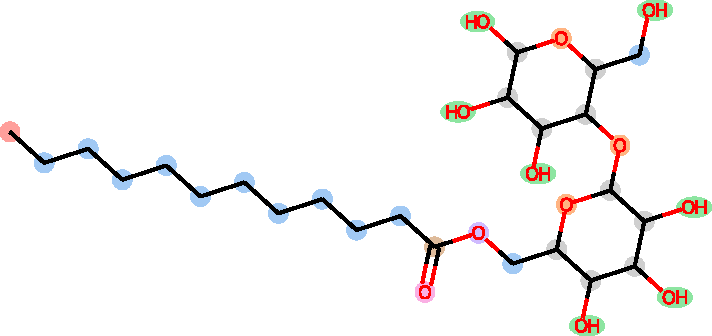
\includegraphics[width=.8\linewidth]{images/molecular-graph.pdf}
    \caption{A molecular graph of 6-\textit{O}-dodecanoyl-maltose. Atoms are
        highlighted based on their feature vectors, $\vec{v}_i$, so that equal
        feature vectors have the same colour.}
    \label{fig:mol-graph}
\end{figure}

\subsection{Model selection}

\subsubsection{ECFP model}

Based on the prior knowledge encoded in Equation~\ref{eq:klevens}, it is
assumed that certain atomic environments have a linear relationship to $\log X_{cmc}$. It therefore seems justified to apply a linear model to the ECFP fingerprints described in Equation~\ref{eq:ecfp}:
\begin{equation}
    \label{eq:linear-ecfp}
    \log X_{cmc} = \vec{w} \cdot \vec{c} + b,
\end{equation}
where $\vec{w}$ is a trained weights vector, the elements of which correspond to the contribution of an atomic environment to the CMC, and $b$ is an intercept (or \emph{bias} term).

However, the issues of the large feature vector size and multicollinearity must
be addressed. To that end, a process of \emph{feature selection} was applied,
whereby a subset of the atomic environments were selected for use in the model.
There are several approaches to feature selection
\cite{liFeatureSelectionData2017}; here, we chose \emph{regularisation} due to
the ease of implementation.

In this approach, we include a term in the loss function that depends on the
norm of $\vec{w}$. The two types of constraints considered are $\ell_1$ and
$\ell_2$ regularisation, which correspond to the inclusion of $\ell_1$ and
$\ell_2$ norms, respectively. Concretely, the ElasticNet
\cite{zouRegularizationVariableSelection2005} loss function was employed:

\begin{equation}
    \label{eq:elastic}
    \min_{\vec{w}} { \frac{1}{2n_{\text{samples}}} \left \Vert \mathbf{C}\vec{w} + \vec{b}- \vec{y} \right \Vert_2 ^ 2 + \alpha\rho \left \Vert \vec{w} \right \Vert_1} + \frac{\alpha(1 - \rho)}{2} \left \Vert \vec{w} \right \Vert_2^2,
\end{equation}

where $n_{\text{samples}}$ is the number of training samples; $\vec{y}$ are the
training data's true values of $\log X_{cmc}$; $\vec{b}$ is a vector with
elements all equal to $b$; and $\alpha$ and $\rho$ are user-defined
hyperparameters describing the degree of regularisation ($\alpha \geq 0$), and
the proportions of the regularisation terms ($0 < \rho < 1$), respectively.
$\mathbf{C}$ are the standardised training data feature vectors,
$\{\vec{c}^{\,\prime}_n \,|\, 1 \leq n \leq n_\text{samples}\}$, stacked
row-wise into a matrix.

Standardising the environment counts ensures that they have zero mean and unit variance:
\begin{equation}
    \label{eq:standard-scaling}
    {c}^{\,\prime}_m = \frac{c_m - u_m}{s_m},
\end{equation}
where $u_m$ and $s_m$ are the mean and standard deviation of the number of
$\mathcal{E}_m$ in each molecule in the training data. This standardisation
ensures that the regularisation term is not dominated by environments with high
variance and that it accounts for common and uncommon environments alike.

By imposing the $\ell_1$ penalty, the model is biased towards learning a
\emph{sparse} weight vector: many of its elements will be negligible. The
corresponding features can be removed from the representation. Meanwhile, the
$\ell_2$ penalty means that a `grouping' effect is achieved, ensuring that
highly correlated groups are assigned similar weights, rather than discarding
some of them. It also ensures that the upper bound on the number of selected
groups is equal to the total number of groups; the model is not constrained to
select a smaller subset if there are no redundant groups. Both of these are
potential issues when using only an $\ell_1$ norm in the loss function
\cite{efronLeastAngleRegression2004,zouRegularizationVariableSelection2005}.

To determine the best values for $\alpha$ and $\rho$, 5-fold cross-validation of
the training data was used. This was applied for a range of $\alpha$ and $\rho$
combinations. The combination that achieved the lowest average
mean-squared-error was used to train a model using the entirety of the training
data. The hyperparameter search space is defined in the Supplementary
Information.

The features with non-negligible fitted weights from ElasticNet were then
selected for use in the final linear model. This model, ridge regression, uses
just $\ell_2$ regularisation so that all of the weights are non-negligible, but
still addresses the issue of multicollinearity
\cite{mcdonaldRidgeRegression2009}:
\begin{equation}
    \min_{\vec{w}} \left \Vert \mathbf{C} \vec{w} + \vec{b} - \vec{y} \right \Vert_2^2 + \alpha \left \Vert \vec{w}\right \Vert_2^2.
\end{equation}
A similar cross-validation method to the one described above was used to
determine the best $\alpha$ parameter, but using leave-one-out cross-validation,
whereby $k=n_\text{samples}-1$. Because only one hyperparameter needs to be
determined, there are far fewer trials per fold and therefore a greater number
of folds can be used.

It was empirically observed that the combination of ElasticNet feature selection and a final regression with the simpler ridge regression model yielded better results, likely due to using a larger number of folds when determining the best value for $\alpha$. Both models were implemented using scikit-learn \cite{pedregosaScikitlearnMachineLearning2011}.

\subsubsection{Molecular graph model}

The basic topology of the graph neural network (GNN) used in this work was
identical to the one used by \citet{qinPredictingCriticalMicelle2021}. The first
step of the model consists of a stack of graph network layers, which mutate the
node features in a molecular graph based on those of bonded atoms. These layers
employ the graph convolution network (GCN) architecture introduced by
\citet{kipfSemiSupervisedClassificationGraph2017}. Layer $l$ computes a new node
feature matrix, $\mathbf{V}^{(l)}$, based on the adjacency matrix, $\mathbf{A}$:
\begin{equation}
    \mathbf{V}^{(l)} = \mathbf{D}^{-\frac{1}{2}} \mathbf{A} \mathbf{D}^{-\frac{1}{2}} \mathbf{V}^{(l-1)} \mathbf{W}^{(l)} + \mathbf{b}^{(l)}.
\end{equation}
Here, $\mathbf{W}^{(l)}$ and $\mathbf{b}^{(l)}$ are the weights and biases,
respectively, of layer $l$. We have also introduced the degree matrix,
\begin{equation}
    D_{ii} = \sum_j A_{ij},
\end{equation}
so that the term $\mathbf{D}^{-\frac{1}{2}} \mathbf{A} \mathbf{D}^{-\frac{1}{2}}$ normalises the
    adjacency matrix based on the degree of each atom.

$\mathbf{V}^{(1)}$, therefore, encodes not only information about the atom itself but its bonded neighbours. This information is used in the subsequent graph convolution so that $\mathbf{V}^{(2)}$ encodes information about the
2\textsuperscript{nd} order neighbourhood, \emph{et cetera}. The number of graphs layers, $L$, therefore dictates the `radius' around each atom that is considered in computing the final feature vector, analogous to creating an ECFP, except that the $i^\text{th}$ atomic environment is characterised by a continuous, \emph{latent} vector, $\vec{v}^{\,(L)}_i$.

The next step is a pooling layer, which converts the graph to a single \emph{latent representation vector}, $\lrv{}$, losing the explicit topological information. Several choices of pooling function were trialled:

\begin{description}
    \item[Mean pooling] was employed by \citet{qinPredictingCriticalMicelle2021}. It computes the average
          over all atoms' latent feature vectors.
    \item[Sum pooling] computes the sum of all atoms' latent feature vectors.
          This is the most analogous to the ECFPs in that the contribution of an atomic environment scales linearly with the number of times it occurs
          in the molecule.
    \item[Gated attention pooling] applies an \emph{attention} mechanism to decide which environments
          are relevant to the prediction \cite{liGatedGraphSequence2017}:
          \begin{equation}
              \lrv{} = \sum_i^N \sigma\left(\mathbf{W}_1 \vec{v}_i^{\,(L)} + \vec{b}_1 \right) \odot \left(\mathbf{W}_2 \vec{v}_i^{\,(L)} + \vec{b}_2 \right),
          \end{equation}
          where $\mathbf{W}_1$ and $\mathbf{W}_2$ are trained weights and
          $\vec{b}_1$ and $\vec{b}_2$ are biases, $\sigma$ is the sigmoid
          activation function, $N$ is the number of atoms in the molecule, and
          $\odot$ represents element-wise multiplication.
    \item[Attention sum pooling] is a simpler variation of the above. By using a
          softmax function, it performs a weighted average of the atomic environments'
          contributions:
          \begin{align}
              \mathbf{X} = \mathrm{softmax}(\mathbf{V}^{(L)}\vec{w}), \\
              \lrv{} = \sum_i^N \mathbf{X}_i \cdot \vec{v}^{\,(L)}_i,
          \end{align}
          where $\vec{w}$ are trained weights.
\end{description}

After training the model, $\lrv{}$ effectively acts as a machine-learned representation of the molecule that captures only the information about its topology and composition that is useful for predicting the CMC. Finding an optimised representation is a feature of neural networks that happens implicitly during training, called \emph{representation learning} \cite{goodfellowRepresentationLearning2016}.
The final step is a readout neural network: a multi-layer perceptron which acts as a nonlinear approximator to map this
latent representation vector to the CMC property prediction. Each layer in this neural network, called a `dense' layer, outputs a new vector, $\vec{v}^{(l)}$:
\begin{equation}
    \vec{v}^{(l)} = \mathbf{W}^{(l)}\vec{v}^{\,(l-1)} + \vec{b}^{\,(l)},
\end{equation}
The full network's architecture is illustrated in
Figure~\ref{fig:model-topology}. The model was implemented using the open-source
library Spektral\cite{grattarolaGraphNeuralNetworks2020} and optimised using an
Adam optimiser \cite{kingmaAdamMethodStochastic2017} to minimise the mean
squared error.

\begin{figure}
    \centering
    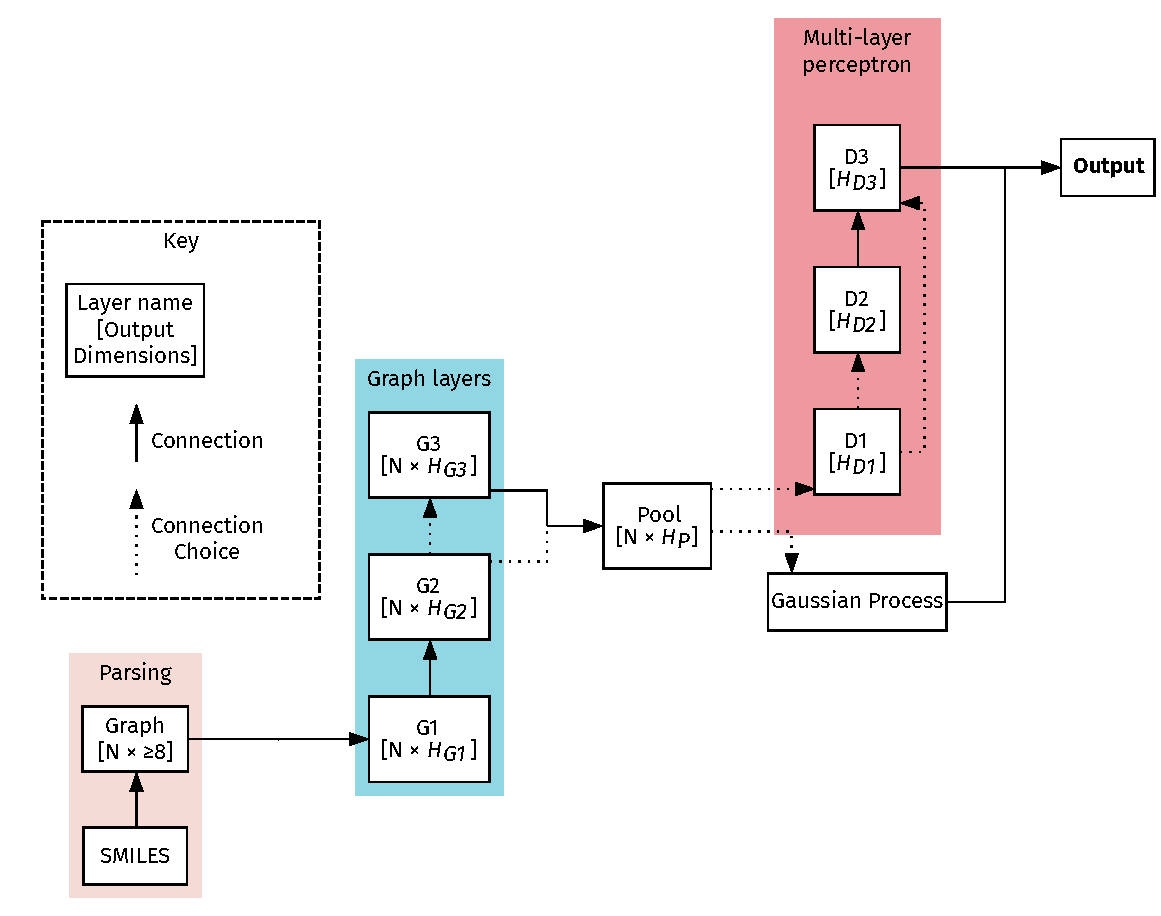
\includegraphics[width=\textwidth]{images/model_graph.pdf}
    \caption{Schematic of the neural network architecture. Here, $N$ represents
        the number of constituent atoms/ions in the input molecule and $H$
        represents a hyperparameter. The size of the pooling layer output, $H_P$, is
        only independent in the case of a gated attention-pooling layer. Otherwise,
        it is equal to the number of columns of the graph layer that feeds into it
        ($H_{G2}$ or $H_{G3}$).}
    \label{fig:model-topology}
\end{figure}

A neural network's topology describes the types of layers used, i.e. their functional form and the connection between them. Layers that are parameterised by a weight matrix, $\mathbf{W}$, may have different `sizes', meaning that the
dimensionality of their output is arbitrary and can be adjusted by changing the dimensions of $\mathbf{W}$. The graph layers, dense layers and the gated attention pool all have this property. These sizes, the type of pooling layer
and the number of each graph and dense layer, are all hyperparameters that can be adjusted prior to training. To determine the best combination of hyperparameters for predicting CMCs, an automated searching procedure was
employed.

\subsubsection{Optimising GNN hyperparameters}

The Hyperband approach \cite{liHyperbandNovelBanditBased2018}, implemented in Keras Tuner \cite{cholletKeras2015}, was used to select a good combination of hyperparameters for the model. Hyperband provides a way to efficiently evaluate
the performance of a large search space of hyperparameter configurations. The algorithm assesses several combinations of hyperparameters, initially allocating only a small number of resources to each trial. The hyperparameters for the
trials with the best performance are then allocated more resources, whilst the remainder is discarded. A reduction factor of 3 was chosen, meaning that $2/3$ of the trials were discarded after each iteration. This procedure iterates until the best configuration is found.

The algorithm can be executed multiple times if resources are available to obtain a more reliable result; the training procedure is stochastic, and therefore the performance of two trials with the same hyperparameters may be different. In this case, a single run was performed. The training data was partitioned into an optimisation subset and a validation subset in a ratio of 9:1. The trials were fit to the optimisation subset and evaluated based on the RMSE of their predictions on the validation subset.
The best hyperparameters determined on the benchmark tasks were then used during the sensitivity analysis.

\subsubsection{Adding uncertainty with a Gaussian process}

To improve the model's reliability, a \emph{surrogate} model was employed that could yield uncertainty estimates alongside CMC predictions. The approach is based on the Convolution-Fed Gaussian Process of \citet{tranMethodsComparingUncertainty2020}. The model first computes the latent representation vector, $\lrv{}$, of an input molecule using a trained GNN. $\lrv{}$ is then standardised, similar to Equation \ref{eq:standard-scaling},
but in this case the standardisation applies across each latent feature, $n$:
\begin{equation}
    v^{(p)\,\prime}_n = \frac{v^{(p)}_n - u_n}{s_n}.
\end{equation}
Again, $u_n$ and $s_n$ were determined from the training molecules' latent representations.

The standardised latent representation vectors of the training data serve as index points for a Gaussian process (GP); see Figure~\ref{fig:model-topology}.
The GP's predicted mean and standard deviation define a predicted normal distribution of a molecule's CMC, $\log X_{cmc} \sim \mathcal{N}(\mu, \sigma)$.

In this work, the GPs  were defined using a Mat\'ern kernel with parameter
$1/2$, and a fixed noise variance of \num{1e-5}. Furthermore, the multi-layer
perceptron component of the GNN used to calculate $\lrv{}$ was employed as the
GP's mean function. The kernel parameters were optimised with an Adam optimiser
\cite{kingmaAdamMethodStochastic2017}. The same optimisation/validation
splitting was used as for the GNN hyperparameter search and training was stopped
after \num{1000} iterations without improvement in the validation predictions'
RMSE, or after a total of \num{5000} iterations. The software implementation was
based on GPFlow \cite{matthewsGPflowGaussianProcess2017}.

\subsubsection{Visualising the latent space}

In order to better understand the model's interpretation of chemical space, we
exploit the GP's kernel, optimised during training, to plot the molecules in 2D
space in a way that respects the model's perception of their `similarity'. This
approach is inspired by \citet{isayevMaterialsCartographyRepresenting2015}, who
compared the fingerprints of several inorganic compounds to develop so-called
materials catrograms. By employing the machine-learned latent representations of
molecules, our cartogram reflects molecular similarities learned by the model
itself.

Having trained the GP, the learned kernel function was computed between every
pair of molecules in the combined data, NIST and Qin. These kernel values were
then normalised within the range $[0, 1]$. Each molecule was assigned a node in
a graph and these were connected by edges. Each edge was given a weight equal to
the normalised kernel value between the two nodes it connected.

This was the starting condition for computing a \emph{force-directed graph
    layout}. The nodes are initialised with a set of 2D coordinates that are
uniformly distributed and they are then moved according to forces acting upon them;
primarily an attractive force that acts along the edges. In addition, there are
pairwise repulsive forces acting amongst the nodes that serves to ensure that
the equilibrium distance between two nodes is non-zero. In this work, the Force
Atlas 2 algorithm was employed
\cite{jacomyForceAtlas2ContinuousGraph2014,bastianGephiOpenSource2009}.

\section{Results}

\subsection{ECFP feature selection}

The number of atomic environments remaining after each stage of the feature
selection process is reported in Table \ref{tab:ecfp-fs}. Notably, the ratio of
the number of features to the size of the training dataset is similar for both
tasks ($\sim \SI{74}{\%}$) and so is the ratio of the initial number of features
to the number of selected features (\SIrange{31}{33}{\%}). The number of
features is large compared to many of the empirical models described above, but
not compared to the number of parameters for the GNN, which is significantly
larger. Because this model also aims to cover a large part of chemical space, a
large number of parameters is to be expected.

\begin{table}
    \centering
    \caption{The number of atomic environments at each stage of the ECFP feature selection process.}
    \label{tab:ecfp-fs}
    \begin{tabular}{@{}lccc@{}} \toprule
                      & \multicolumn{3}{c}{Number of training data atomic environments}                                                            \\\cmidrule(l){2-4}
        Task          & Initially                                                       & Found in multiple molecules & With non-negligible weight \\\midrule
        Qin-Nonionics & 260                                                             & 201                         & 81                         \\
        Qin-All       & 410                                                             & 302                         & 134                        \\\bottomrule
    \end{tabular}
\end{table}

The OPTICS clustering routine on the Qin-All dataset using these fingerprints
resulted in 24 classes and 31 outlying molecules. The resulting classifications
for each molecule are available in the Supplementary information.

\subsection{Hyperband tuning}

\num{725} trials were conducted for each of the Qin training datasets. The best
hyperparameters discovered on each set are described in Table \ref{tab:hb-hps}.

\begin{table}
    \centering
    \caption{The best hyperparameters discovered during searching. The $H$
        values refer to the dimensions of the corresponding layer, see Figure
        \ref{fig:model-topology}. Values for $H_{G3}$ and $H_{D2}$ have been
        omitted where the layers were not included in the model, and the values
        of $H_P$ were only independent for the gated attention pool, so that
        they are omitted here as well.}
    \label{tab:hb-hps}
    \begin{tabular}{@{}lcc@{}} \toprule
                        & \multicolumn{2}{c}{Best value for}            \\\cmidrule(l){2-3}
        Hyperparameter  & Qin-Nonionics                      & Qin-All  \\\midrule
        \# Graph layers & 2                                  & 3        \\
        $H_{G1}$        & 320                                & 64       \\
        $H_{G2}$        & 256                                & 64       \\
        $H_{G3}$        & --                                 & 128      \\
        Pooling layer   & Mean pool                          & Sum pool \\
        $H_P$           & --                                 & --       \\
        \# Dense layers & 2                                  & 2        \\
        $H_{D1}$        & 128                                & 256      \\
        $H_{D2}$        & --                                 & --       \\\bottomrule
    \end{tabular}
\end{table}

\subsection{Benchmark model performance}

The performances of all the trained models on the benchmark tasks are reported
in Table \ref{tab:evaluation}. All of the models developed here outperformed
those of \citet{qinPredictingCriticalMicelle2021}. For every task, the most
accurate model was either the GNN or the combined GNN with GP (GNN/GP). The
linear model's performance is surprisingly good, considering its relative
simplicity, faster optimisation and the far smaller number of parameters it
constitutes.

\begin{table}
    \centering
    \caption{Benchmark task evaluation results for the models trained in this work versus those of the previous work. The best RMSE for each task is emboldened.}
    \label{tab:evaluation}
    \begin{tabular}{@{}lccc@{}} \toprule
                                                              & \multicolumn{3}{c}{Test RMSE (\si{\log \micro M})}                                 \\\cmidrule(l){2-4}
        Model                                                 & Qin-Nonionics                                      & Qin-All       & NIST          \\\midrule
        Previous work \cite{qinPredictingCriticalMicelle2021} & 0.23                                               & 0.30          & --            \\
        ECFP                                                  & 0.19                                               & 0.26          & 1.57          \\
        GNN                                                   & \textbf{0.15}                                      & 0.29          & 1.35          \\
        GNN/GP                                                & 1.38                                               & \textbf{0.21} & \textbf{1.32} \\\bottomrule
    \end{tabular}
\end{table}

As expected, the performance of all models on the NIST data is significantly
worse than on the test data. This supports the hypothesis that the NIST data
molecules are outside of the applicability domain of the models developed here,
but it does not exclude the possibility that the models are instead overfitted.
Therefore, a more detailed analysis of the applicability domain will be provided
below.

Finally, it is noted that the GNN/GP model's predictive performance on the
Qin-Nonionics task was very poor. This indicates that the spacing between the
molecules' latent representation vectors, determined from the corresponding GNN,
was not a good indicator of similarity with respect to CMC prediction.

\subsubsection{Uncertainty quantification}

The RMSE alone does not capture the quality of the predicted standard
deviations. One metric that captures these is the negative log-likelihood (NLL)
of observing the true CMCs, given the model's predicted normal distributions:
\begin{equation}
    \text{NLL} = -\sum_n \log p_n(\hat{y}_n),
\end{equation}
where subscript $n$ is the index of the data, $\hat{y}_n$ is the true CMC value and $p_n$ is the probability density function of the normal distribution $\mathcal{N}(\mu_n, \sigma_n)$, where $\mu_n$ and $\sigma_n$ are the predicted
mean and standard deviation. This metric indicates the relative performance of different models on the same data. (Note that its value scales with the size of the data.) It does not give a good indication of the quality of any individual
model in isolation, however. The NLL values are included in the supplementary information for comparison against future work.

To assess the models' quality individually, the predictions can be visualised
against the true CMCs in a parity plot; see Figure~\ref{fig:uq-parity}.
Alternatively, a calibration plot can be used, which compares the cumulative
distribution of the residuals against the expected distribution, given a model's
predicted standard deviations. The expected distribution stipulates what would
be observed if the residuals were drawn from the distributions predicted by the
corresponding model. Deviations from this distribution indicate whether the
model was over- or underconfident (c.f.
\citet{tranMethodsComparingUncertainty2020}). The calibration plots are shown in
Figure~\ref{fig:uq-calibration}.

\begin{figure}
    \centering
    \begin{subfigure}{\textwidth}
        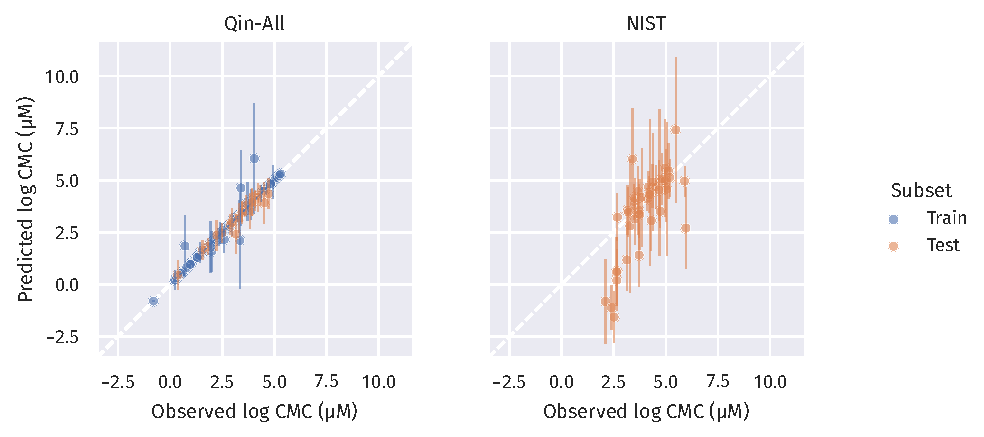
\includegraphics[width=\textwidth]{images/uq-parity.pdf}
        \caption{}
        \label{fig:uq-parity}
    \end{subfigure}
    \begin{subfigure}{\textwidth}
        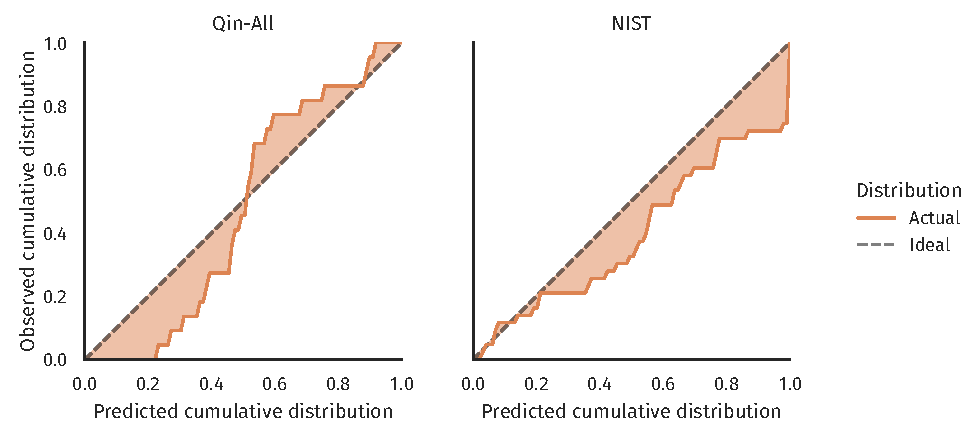
\includegraphics[width=\textwidth]{images/uq-calibration.pdf}
        \caption{}
        \label{fig:uq-calibration}
    \end{subfigure}
    \caption{(a) Parity plots of the predicted CMCs from the GNN/GP model and \SI{95}{\%}
        confidence intervals for the Qin-All and NIST datasets and (b)
        corresponding calibration plots for the test data predictions. The
        `ideal' distribution line indicates the cumulative distribution that
        would be obtained if residuals were drawn from the model's predicted
        distributions.}
\end{figure}

The S-shaped calibration curve for the Qin-All test data indicates that the
model was underconfident in its predictions. In fact, there is a spike in the
number of observed residuals that are close to the centre of the distribution.
The corresponding parity plot shows that the predicted uncertainties were
relatively small. The NIST data calibration curve's asymmetry indicates its
tendency to underestimate the CMCs. It shows a generally good agreement with the
ideal distribution, with the greatest discrepancy above \num{0.8}, which
indicates that there are several surfactants whose CMC predictions are too low
and that these predictions are overconfident, i.e. their predicted standard
deviations are too small.

\subsection{ECFP interpretations}

The weights of the ECFP models are coefficients corresponding to the scaled counts of the selected atomic environments. Referring to Equations \ref{eq:linear-ecfp} and \ref{eq:standard-scaling}, these coefficients indicate
the change in a predicted CMC when the count of $\mathcal{E}_m$ increases by $s_m$ from its average, $u_m$. A more readily interpreted value can be achieved by rescaling the coefficient, $w_m$, for an environment:
\begin{equation}
    w_m^\prime = \frac{w_m(1 - u_m)}{s_m},
\end{equation}
which indicates the difference in predicted CMC between a molecule containing
one $\mathcal{E}_m$ and a molecule without any $\mathcal{E}_m$, but which
otherwise contains exactly the same number as all the other environments. This
scaled weight can be interpreted as a rough indication of the relative
importance of different environments to determining CMC; `rough' because it may
not be physically plausible that two molecules exist that are distinguished only
by the number of $\mathcal{E}_m$ that they contain. This is particularly true of
larger environments that envelope smaller ones. The largest scaled weights for
the two ECFP models are given in Table \ref{tab:env-coefs}.

\begin{table}
    \centering
    \caption{The atomic environments with the greatest importance to CMC according to the trained ECFP models.}
    \label{tab:env-coefs}
    \begin{tabular}{@{}lSlS@{}} \toprule
        \multicolumn{2}{c}{Qin-All}                 & \multicolumn{2}{c}{Qin-Nonionics}                                                                                                                      \\\cmidrule(r){1-2}\cmidrule(l){3-4}
        Environment                                 & {Scaled weight}                   & Environment                                                                                      & {Scaled Weight} \\\midrule
        \ce{(CH2)5}                                 & -0.64                             & \ce{(CH2)5}                                                                                      & -0.76           \\
        \ce{(CH2)3}                                 & -0.55                             & \ce{(CH2)3}                                                                                      & -0.69           \\
        \ce{Cl-}                                    & 0.31                              & \chemfig{-[1]-[-1](-[-3]R_1)-[1]R_2}                                                             & -0.29           \\
        \ce{Br-}                                    & 0.29                              & \chemfig{R_1-[1](-[-1]R_3)-[3]R_2}                                                               & -0.25           \\
        \chemfig{R_1-[1]-[-1]-[1](-[3]R_2)-[-1]R_3} & -0.27                             & \chemfig{R_1-[1](-[4]R_2)(-[-2]R_3)-[1](-[3]OH)-[-1](-[-3]OH)-[1](-[3]OH)-[-1](-[-3]R_4)-[1]R_5} & -0.19           \\
        \ce{CH2}                                    & -0.23                             & \chemfig{R_1-[-1]-[1](-[3]OH)-[-1](-[-3]OH)-[1](-[3]OH)-[-1](-[-3]R_2)-[1]R_3}                   & 0.14            \\
        \ce{R1-O-R2}                                & 0.18                              & \chemfig{R_1-[-1](-[-3]R_2)-[1](-[3]OH)-[-1](-[-3]OH)-[1]-[-1]OH}                                & -0.12           \\
        \ce{OH}                                     & -0.17                             & \chemfig{R_1-[-1]-[1](=[3]O)-[-1](-[-3]OH)-[1](-[3]OH)-[-1]}                                     & 0.09            \\
        \ce{R1-O-(CH2)2OH}                          & -0.14                             & \ce{CH3}                                                                                         & -0.06           \\
        \ce{CH2-O-(CH2)2OH}                         & -0.14                             & \chemfig{R_1-[-1](-[-3]R_2)-[1](-[3]OH)-[-1](-[-3]OH)-[1](-[3]OH)-[-1](-[-3]R_3)-[1]R_4}         & 0.05            \\
        \bottomrule
    \end{tabular}
\end{table}

Both the Qin-Nonionic and Qin-All models agree that alkyl chain environments
constitute the top two most important contributors to CMC, suggesting that tail
length is the most important factor. The model trained on all surfactant classes
includes two counterions in its most important environments: \ce{Cl-} and
\ce{Br-}. This is to be expected; ionic surfactants typically have much larger
CMCs than nonionics, and the model appears to distinguish these by their
counterion. The Qin-Nonionics model identifies environments from the headgroups
of sugar-based surfactants as being important. These surfactant headgroups
possessed relatively complex topologies and therefore several environments; it
may have been necessary for the model to use many of these environments in order
to accurately distinguish between their CMCs.

\subsection{Applicability domain analysis}

Several of the molecules included in the NIST dataset were expected to be outside
of the applicability domain, which justifies their poor prediction accuracy. The
majority of the outliers' CMCs are underpredicted, and the GNN/GP model is
overconfident in their predictions. The 13 surfactants whose predictions'
residuals are greater than the \SI{95}{\%} confidence interval (CI) are shown in
Figure~\ref{fig:nist-underpred}. These constitute 3 nonionic surfactants, 1
zwitterionic surfactant and 9 ionic surfactants. Of the ionic surfactants, 5
have quaternary ammonium salts (quats) as counterions.

\begin{figure}
    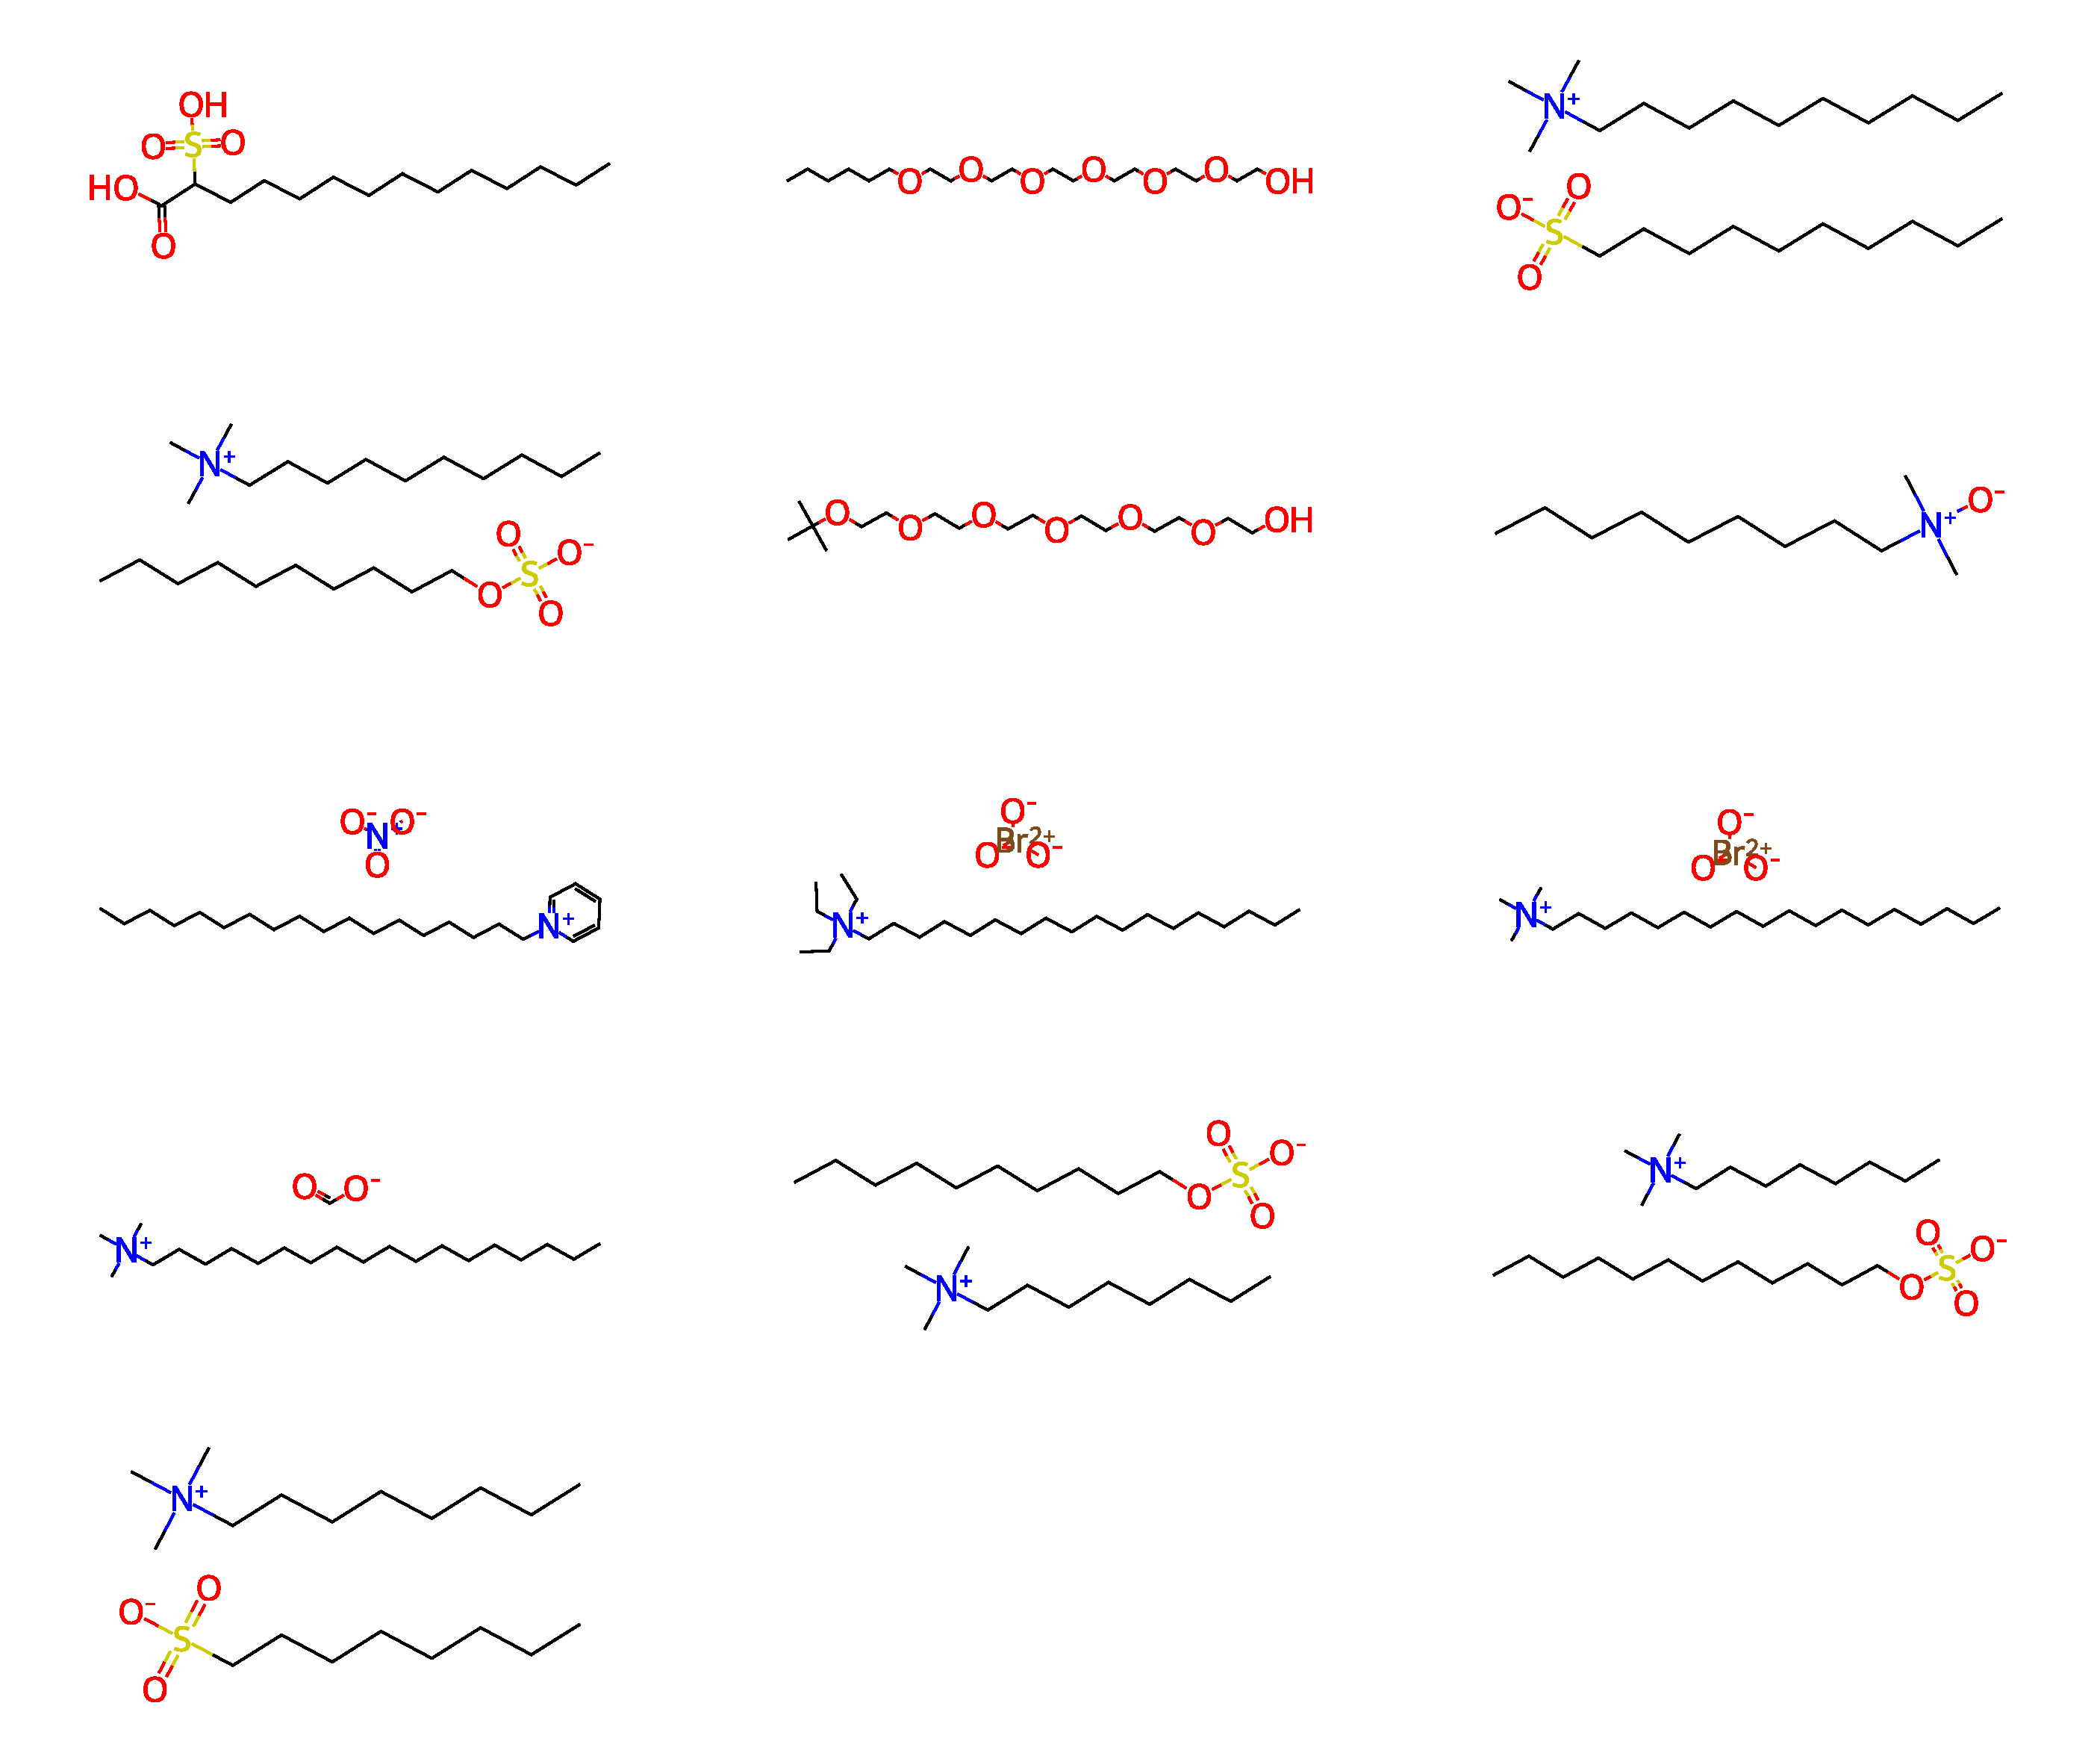
\includegraphics[width=\textwidth]{images/nist-underpred.pdf}
    \caption{The 13 surfactants and counterions in the NIST dataset with residuals
        that were greater than the \SI{95}{\%} confidence interval.}
    \label{fig:nist-underpred}
\end{figure}

It is useful to examine the types of counterions in these molecules as compared
to the training data. In the training data, there are no examples with a
bromate, nitrate or carbonate counterion, but there are two examples of a quat
counterion. However, the quats in the training data are isotropic:
tetrapropylammonium and tetramethylammonium. In contrast, those that are
underpredicted are highly anisotropic and are effectively surfactants
themselves; the behaviour of these compounds, in terms of CMC, can be expected
to be very different to that of the surfactants in the training data.
Furthermore, the two polyoxyethylene alcohols in Figure~\ref{fig:nist-underpred}
have remarkably small tail groups relative to the examples in the training data,
which justifies their erroneous CMC predictions. This leaves two surfactants
among the outliers that might reasonably be expected to lie within the
applicability domain, constituting \SI{4.7}{\%} of the total NIST dataset, which
is close to the \SI{5}{\%} that are expected to be outside the \SI{95}{\%} CI.

To gain insight into the relationships between molecules, we exploit the kernel
function from the trained GP to create a molecular cartogram, as explained in
the Method. The resulting cartogram is shown in Figure~\ref{fig:fdg}. The NIST
molecules whose residuals are above the \SI{95}{\%} CI are also highlighted
separately.

From the cartogram of the entire data, it is apparent that the majority of the
surfactants are segregated based upon the type of counterion in the solution.
This suggests that the model has learned that the counterion is an important
factor for determining CMC and the weights associated with this counterion have
a profound impact on the CMC prediction. However, the visualisation of the NIST
molecules with CMCs above the \SI{95}{\%} CI indicates that the model classifies
all of these molecules as being primarily similar to the nonionic or
zwitterionic compounds. This is clearly erroneous for the ionic compounds: the
quats, the bromates, the carbonates and the nitrates. This suggests that the
model has not learned appropriate weights for these counterions, hence it fails
to properly segregate them.

\begin{figure}
    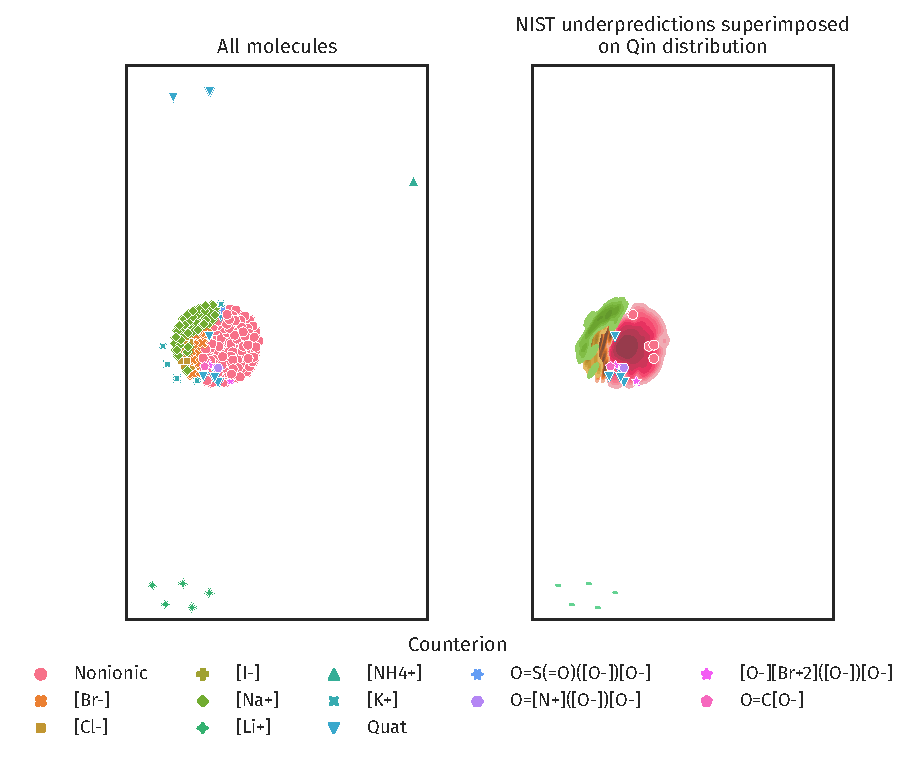
\includegraphics[width=\textwidth]{images/force-graph.pdf}
    \caption{Cartogram of the molecules in the combined NIST and Qin datasets
        using a force-directed graph layout. Left: The entirety of the combined
        NIST and Qin datasets, where each molecule is assigned a point. Right:
        The NIST molecules that are overconfidently underpredicted, so that the
        residual is above the \SI{95}{\%} confidence interval, are superimposed
        on a kernel density estimate (KDE) plot of the Qin data. This KDE plot
        is an estimate of the distribution of the Qin molecules on the left,
        coloured by the type of counterion.}
    \label{fig:fdg}
\end{figure}

\subsection{Sensitivity analysis}

Figure~\ref{fig:sensitivity} shows the test set evaluations for the GNN and ECFP
models using repeated, stratified $k$-fold cross-validation. The ECFP and GNN
models show very similar performance on the Qin-All dataset, but the ECFP model
outperforms the GNN model for all training ratios on the Qin-Nonionics dataset.
This is indicative of the propensity of neural networks to overfit, especially
on such small dataset sizes. Notably, there is also a much broader distribution
of RMSEs on the Qin-Nonionics data. This suggests that both of the Qin-Nonionics
models are much more sensitive to the specific molecules that are included in
the train and test splits.

Extrapolating the trend lines indicates that the benchmark performance is much
better than what would be expected. This highlights the importance of selecting
an appropriate training data split, which spans the entirety of the chemical
space of interest. On a dataset as small as the one used here, it is not
possible to achieve this without using a high training ratio.

\begin{figure}
    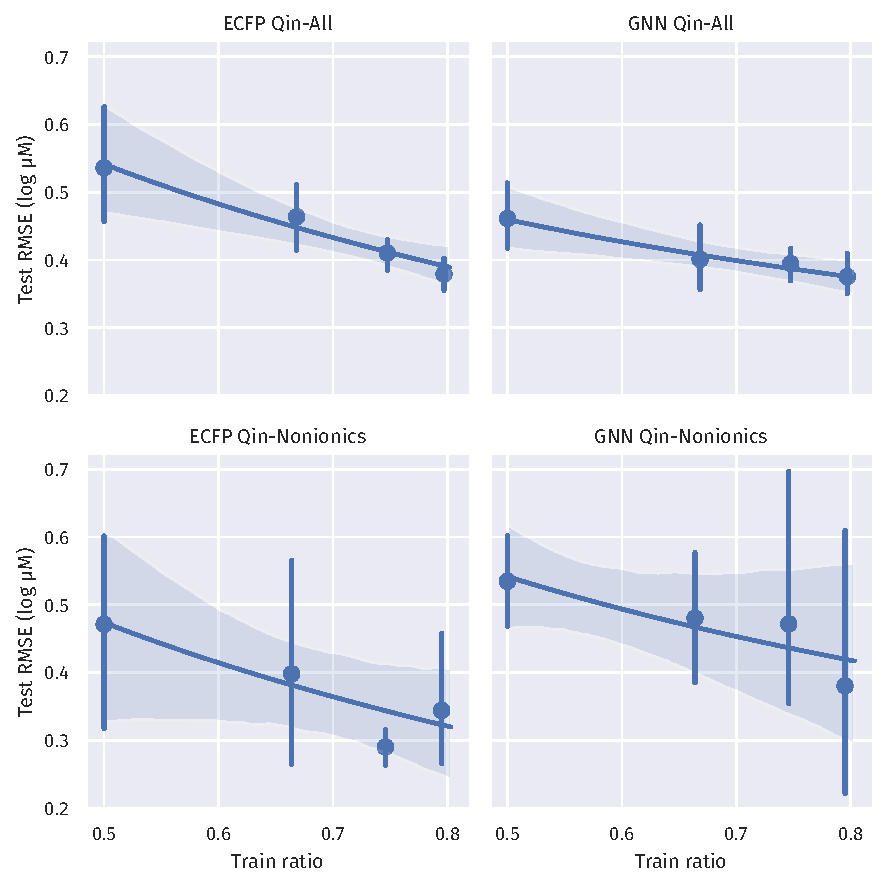
\includegraphics[width=\textwidth]{images/sensitivity-plots.pdf}
    \caption{Test set RMSEs for the sensitivity analysis models. The average
        RMSE for each value of $k$ is indicated, as well as the range of the RMSEs.
        A logarithmic fit to the data is shown, with a \SI{95}{\%} confidence
        interval determined by bootstrapping, using \num{1000} repeats.}
    \label{fig:sensitivity}
\end{figure}

\section{Discussion}

The ideal molecular
representation depends on the task at hand. Ideally, it should be compact but
complete
\cite{faberCrystalStructureRepresentations2015,himanenDScribeLibraryDescriptors2020};
`as simple as possible, but not simpler.' To that end, the representation should
contain enough information to distinguish between isomers that with distinct
properties. However, concessions can be made if we restrict the model's domain
and self-imposed limits on the type of isomers we expose the model to, both
during training and in use. Representations may also include descriptions of
state, such as temperature and pressure \cite{chenGraphNetworksUniversal2019},
but this is redundant in cases where the training data spans a very limited
range of states.

The representations employed by both the GNN and the linear models capture
topological information and the performances of all of the models on in-domain
data suggest that this is sufficient for the task of predicting CMC very
accurately. However, both of the models are unable to distinguish between
certain positional isomers, depending on the size of the atomic environments
that they consider. In the case of ECFPs, this is dictated by the radius around
each atom that is included in the fingerprint, whilst for the GNNs, this is
determined by the number of consecutive graph layers.

Increasing these parameters both increases computational cost and model
complexity, introducing more parameters and therefore requiring more data in
order to optimise them appropriately. The sensitivity analysis demonstrated that
this also increases the propensity for overfitting; however, the benchmarking
results demonstrate that using a proper selection of training samples can yield
more accurate models. In cases where there are fewer samples available, and some
chemical classes are poorly represented in the training data, the simpler,
linear model may be preferable.

One of the great advantages of using such a topological approach is that the
contributions of each molecular fragment can be explicitly determined, as shown
in the section on ECFP interpretations. In the case of the GNN, introducing a
kernel to the model, via a Gaussian process operating on the GNN's learned
latent space representations, offers a quantitative measure of molecular
similarity that can simultaneously be employed for adding uncertainty to the CMC
predictions and visualising the chemical space of the training data.
Superimposing the test data onto this cartogram highlights which molecules may
have erroneous predictions, based on the fact that they are clustered amongst
training data molecules with very different chemistries.

Case-by-case examination of these molecules highlights the nature of these chemical
differences, which can be related to properties that are important for micellisation.
Broadly speaking, the model failed in three cases:
\begin{itemize}
    \item Where ionic effects of the solute were not learned, as in the case of the counterions that were unique to the NIST data.
    \item When there was a significant difference in hydrophilic-lipophilic balance (HLB), as in the case of the surfactants with very small tail groups.
    \item When the counterion was itself surfactant-like, as in the case of the
          quats, which implies the system should better be described as a binary
          mixture of surfactants.
\end{itemize}
These results stress the importance of applying domain knowledge in developing
and analysing the results of deep learning models. The uncertainty
quantification is unreliable when the systems' behaviour is starkly different
from what the model can be expected to learn from the training data.

Future efforts to improve this type of model may consider incorporating another
term in the loss function for the GNN that explicitly biases the model towards
learning a form of $\lrv{}$ that captures chemical similarity based on
user-defined metrics; for example, HLB of the surfactant and its counterion.
This approach would enable chemical knowledge to be explicitly encoded within
the model and may capture some of the aforementioned failure cases.
Alternatively, a variational Gaussian process could be used, which approximates
the Gaussian process using a fixed-size set of `pseudo-points'
\cite{hensmanGaussianProcessesBig2013}; this would enable the entire GNN/GP
model to be trained at once using backpropagation and can be applied when the
training data size is larger
\cite{moriartyUnlockNNUncertaintyQuantification2022}.

\section{Conclusions}

Empirical models were developed and applied to predict CMCs from two datasets of
aqueous surfactants. One dataset was partitioned into training and test data
(Qin-All), and a subset of the nonionic surfactants within this data was also
used as a separate prediction task (Qin-Nonionics). The NIST dataset was
collected from a different source and contained molecules with somewhat
different chemistries than the above.

A linear model based on ECFPs demonstrated remarkably good performance,
improving on a previous work \cite{qinPredictingCriticalMicelle2021} that
applied a more complex GNN model, despite using a smaller number of parameters
and having a much faster optimization time. A new model was presented that
improved the architecture of previous work's GNN using a hyperparameter search
algorithm, which was capable of obtaining better performances than the ECFP
model on the Qin-Nonionics task and demonstrated a better ability to generalize
to the NIST dataset.

Sensitivity analysis showed that the GNN models have a tendency to overfit when
training data samples do not adequately cover the chemical space of interest.
When using small datasets, with only a few examples of certain surfactant
classes, our analysis suggests that it may be preferable to use a simpler
functional form, like the linear ECFP model.

A surrogate model was developed by feeding the latent space representation of a
molecule, learned by the GNN model, to a Gaussian process. This yielded
uncertainty estimates alongside CMC predictions. Although this model failed when
applied to the Qin-Nonionics task, it yielded the best predictive performance of
all of the models trained here for the Qin-All task, as well as providing good
uncertainty estimates on the in-domain NIST test data. This approach would allow
practitioners to gauge their confidence in the model's predictions for systems
within the applicability domain.

Finally, the kernel function that is learned while training the Gaussian process
was employed to visualize the chemical space using a molecular cartogram. By
analyzing this cartogram, it was shown that chemical intuition could be employed
to determine which molecules were likely poorly represented in the latent space,
based on the fact that they were surrounded by molecules with different
chemistries. This proves to be a useful technique for exploring the limits of a
model's applicability domain, as well as understanding why the model yields its
predictions for a given molecule based on proximity to training set molecules
within the cartogram.

This work demonstrates the potential of Gaussian processes to add uncertainty
quantification to machine learning models with minimal overhead. There is still
scope to overcome the limitations of these models with respect to small
datasets, such as Qin-Nonionics, and out-of-domain molecules, which could be
achieved by explicitly biasing the latent space.

%%%%%%%%%%%%%%%%%%%%%%%%%%%%%%%%%%%%%%%%%%%%%%%%%%%%%%%%%%%%%%%%%%%%%
%% The "Acknowledgement" section can be given in all manuscript
%% classes.  This should be given within the "acknowledgement"
%% environment, which will make the correct section or running title.
%%%%%%%%%%%%%%%%%%%%%%%%%%%%%%%%%%%%%%%%%%%%%%%%%%%%%%%%%%%%%%%%%%%%%
\begin{acknowledgement}
We thank the Advanced Characterisation of Materials CDT and the ABK fellowship
for their financial support. This work was supported in part by the Engineering
and Physical Sciences Research Council (EPSRC), project number EP/VO32909/1. AS
gratefully acknowledges financial support from the Asahi Glass Chair of Chemical
Engineering at the University of Oklahoma. All the authors are grateful to
Innospec Ltd. for their support.
\end{acknowledgement}

%%%%%%%%%%%%%%%%%%%%%%%%%%%%%%%%%%%%%%%%%%%%%%%%%%%%%%%%%%%%%%%%%%%%%
%% The same is true for Supporting Information, which should use the
%% suppinfo environment.
%%%%%%%%%%%%%%%%%%%%%%%%%%%%%%%%%%%%%%%%%%%%%%%%%%%%%%%%%%%%%%%%%%%%%
\begin{suppinfo}

    Source code for featurization and model training, graph neural network logs
    and metrics for hyperparameter optimization and final training, and
    individual model predictions is available at
    \url{https://github.com/a-ws-m/CaMCaNN/}.

\end{suppinfo}

%%%%%%%%%%%%%%%%%%%%%%%%%%%%%%%%%%%%%%%%%%%%%%%%%%%%%%%%%%%%%%%%%%%%%
%% The appropriate \bibliography command should be placed here.
%% Notice that the class file automatically sets \bibliographystyle
%% and also names the section correctly.
%%%%%%%%%%%%%%%%%%%%%%%%%%%%%%%%%%%%%%%%%%%%%%%%%%%%%%%%%%%%%%%%%%%%%
\bibliography{camcann.bib}

\end{document}